\documentclass[aspectratio=169, 10pt]{beamer}

% --- PACKAGES ---
\usepackage{amsmath}
\usepackage{booktabs}
\usepackage{graphicx}
\usepackage{tikz}
\usetikzlibrary{arrows.meta, positioning, shapes.geometric, calc, backgrounds, fit}

% --- GRAPHICS PATH ---
\graphicspath{{Wang_Active_Acquisition/figures/}{Wang_Active_Acquisition/report_images/}}

% --- COLOR DEFINITIONS ---
\definecolor{Garnet}{HTML}{73000A}
\definecolor{GarnetDark}{HTML}{500007}
\definecolor{Rose}{HTML}{CC2E40}
\definecolor{Atlantic}{HTML}{466A9F}
\definecolor{Congaree}{HTML}{1F414D}
\definecolor{Horseshoe}{HTML}{65780B}
\definecolor{Black90}{HTML}{363636}
\definecolor{Black70}{HTML}{5C5C5C}
\definecolor{Black30}{HTML}{C7C7C7}
\definecolor{Black10}{HTML}{ECECEC}

% --- BEAMER THEME SETTINGS ---
\usetheme{default}
\setbeamertemplate{navigation symbols}{}
\setbeamertemplate{blocks}[default]
\setbeamertemplate{itemize items}[square]
\setbeamertemplate{enumerate items}[square]

% --- DISABLE ROUNDED CORNERS ---
\setbeamertemplate{rounded}{}

% --- COLOR THEME ---
\setbeamercolor{structure}{fg=Garnet}
\setbeamercolor{frametitle}{fg=white, bg=Garnet}
\setbeamercolor{title}{fg=white, bg=Garnet}
\setbeamercolor{alerted text}{fg=Rose}
\setbeamercolor{block title}{fg=white, bg=Horseshoe}
\setbeamercolor{block body}{fg=Black90, bg=Black10}
\setbeamercolor{itemize item}{fg=Garnet}
\setbeamercolor{enumerate item}{fg=Garnet}

% --- FOOTLINE ---
\setbeamertemplate{footline}{
  \leavevmode%
  \hbox{%
  \begin{beamercolorbox}[wd=.333\paperwidth,ht=2.5ex,dp=1ex,left]{footline}%
    \hspace{0.5em}\footnotesize AIAA Region II Student Conference 2026
  \end{beamercolorbox}%
  \begin{beamercolorbox}[wd=.334\paperwidth,ht=2.5ex,dp=1ex,center]{footline}%
    \footnotesize University of South Carolina
  \end{beamercolorbox}%
  \begin{beamercolorbox}[wd=.333\paperwidth,ht=2.5ex,dp=1ex,right]{footline}%
    \footnotesize\insertframenumber{}/\inserttotalframenumber\hspace{0.5em}
  \end{beamercolorbox}}%
  \vskip0pt%
}
\setbeamercolor{footline}{fg=Black70, bg=Black10}

% --- FRAMETITLE CUSTOMIZATION ---
\setbeamertemplate{frametitle}{
  \nointerlineskip
  \begin{beamercolorbox}[wd=\paperwidth,ht=2.5ex,dp=1ex]{frametitle}
    \hspace{0.5em}\insertframetitle
  \end{beamercolorbox}
}

% --- TITLE INFORMATION ---
\title{Dual-Camera Active Acquisition for Automated Small-Object Dataset Construction}
\author{J. Wang, J.C. Vaught, D. Cahl, Y. Wang}
\institute{Department of Mechanical Engineering\\University of South Carolina}
\date{AIAA Region II Student Conference 2026}

\begin{document}

% --- TITLE SLIDE ---
{
\setbeamercolor{background canvas}{bg=Garnet}
\setbeamercolor{normal text}{fg=white}
\usebeamercolor[fg]{normal text}
\begin{frame}[plain]
\vfill
\begin{center}
{\Large\textbf{Dual-Camera Active Acquisition for Automated Small-Object Dataset Construction}}\\[1em]
{\normalsize J. Wang, J.C. Vaught, D. Cahl, Y. Wang}\\[0.5em]
{\small Department of Mechanical Engineering\\University of South Carolina}\\[1.5em]
{\footnotesize AIAA Region II Student Conference 2026}
\end{center}
\vfill
\end{frame}
}

% --- SLIDE 1: MOTIVATION ---
\begin{frame}{Motivation: The Small-Object Detection Bottleneck}
\begin{columns}[T]
\column{0.5\textwidth}
\textbf{Problem:}
\begin{itemize}
\item Small objects in wide-angle views occupy \textasciitilde{}15$\times$15 pixels
\item Insufficient detail for classification
\item Distractors indistinguishable from targets
\end{itemize}

\vspace{0.5em}
\textbf{Existing Approaches:}
\begin{itemize}
\item \alert{Digital zoom:} Magnifies ambiguity, no new information
\item \alert{Super-resolution:} Generative, risk of hallucination, 300+ ms latency
\item \alert{Single high-res camera:} Prohibitive GPU memory for 4K/8K real-time
\end{itemize}

\column{0.5\textwidth}
\begin{figure}
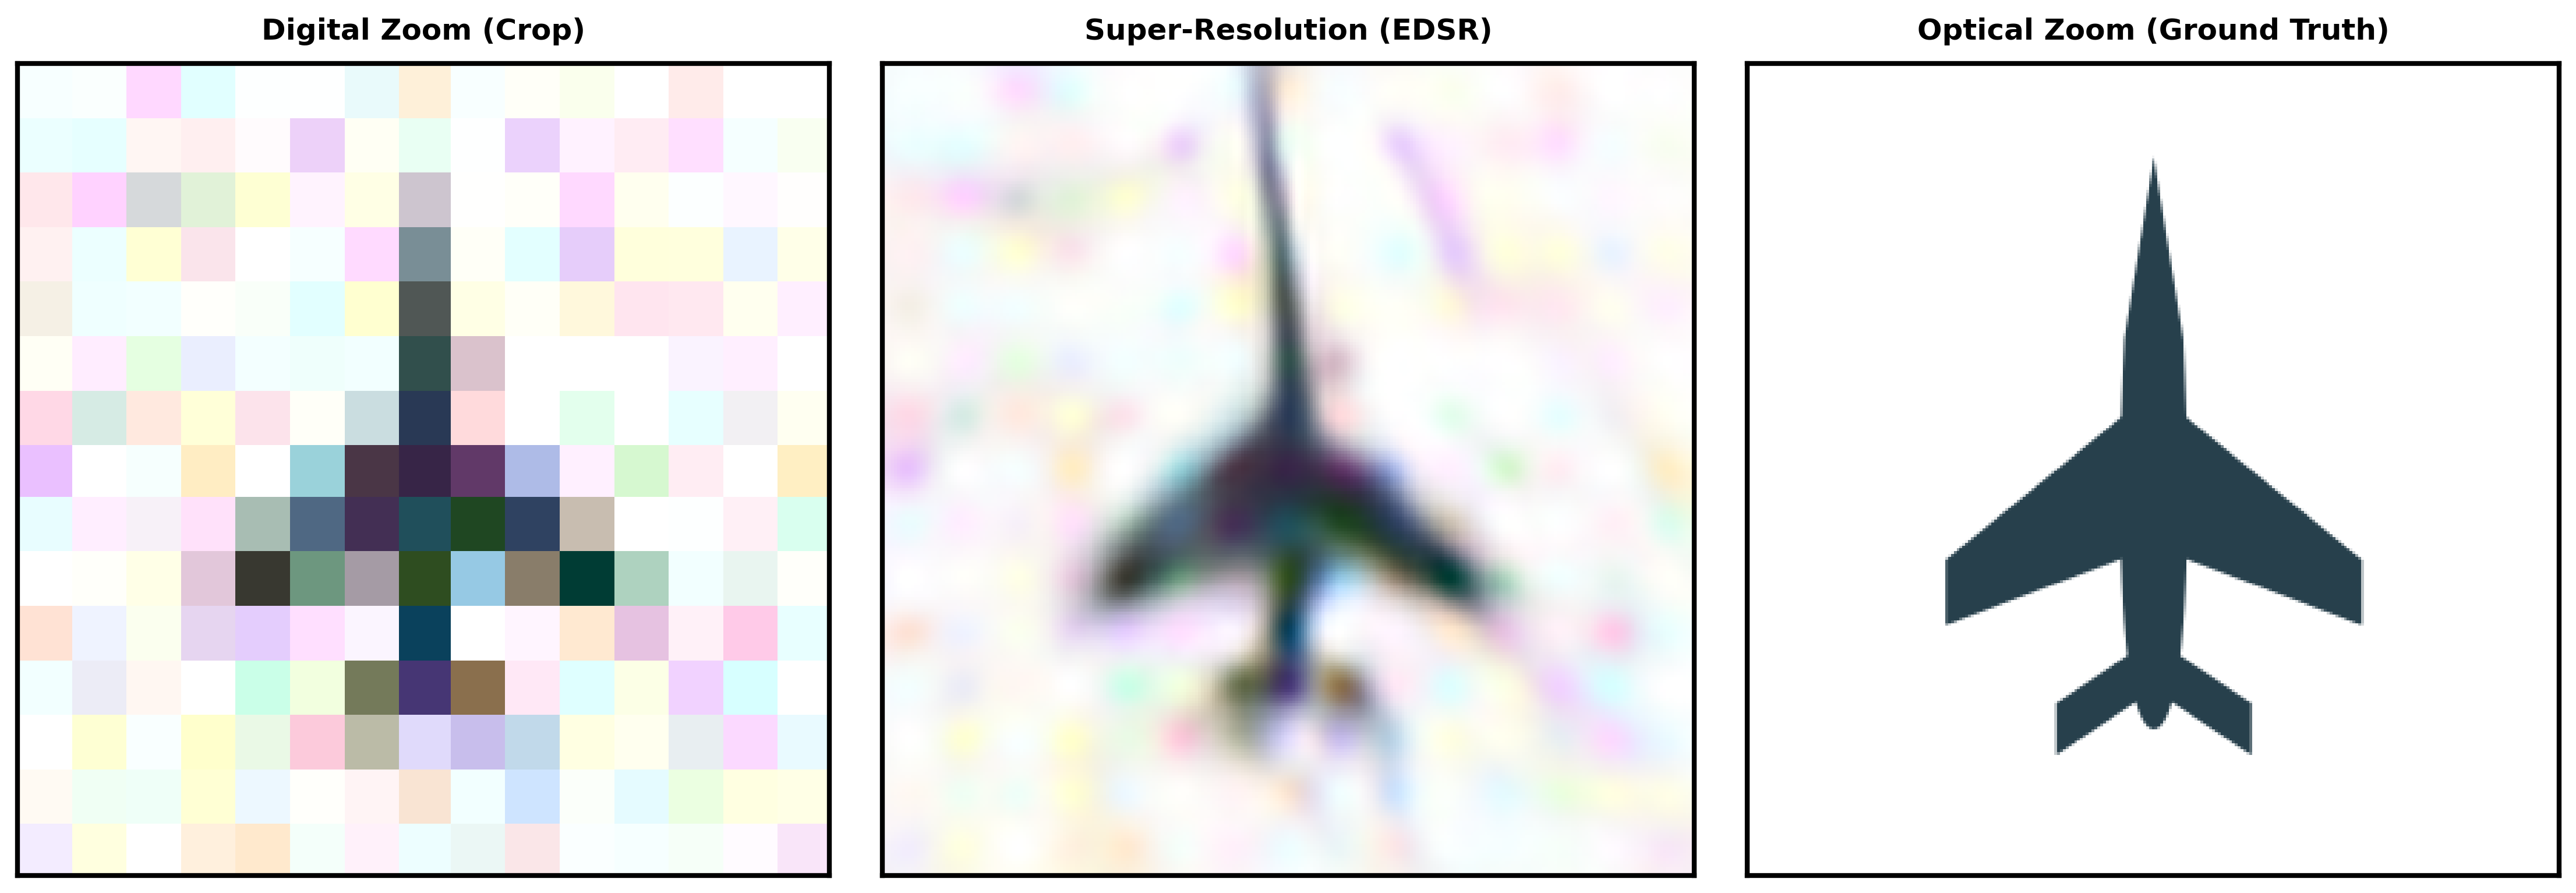
\includegraphics[width=\textwidth]{fig_sr_comparison.png}
\caption*{\scriptsize Wide-angle crop vs super-resolution vs optical zoom}
\end{figure}
\end{columns}

\vspace{0.5em}
\textbf{\textcolor{Horseshoe}{Our Solution:}} Replace digital zoom and SR with \emph{optical zoom} via dual-camera active acquisition
\end{frame}

% --- SLIDE 2: SYSTEM HARDWARE OVERVIEW ---
\begin{frame}{System Hardware Overview}
\begin{columns}[T]
\column{0.5\textwidth}
\textbf{Hardware Configuration:}
\begin{itemize}
\item 2$\times$ FLIR M300C cameras
\item Baseline separation: 0.5 m
\item Parallax at 100 m: 0.29$^\circ$ (negligible)
\item Power: 12.8 V 50 Ah LiFePO4 battery
\item Compute: NVIDIA Jetson Orin AGX
\item JetPack 4.7, CUDA 12.6
\item PCIe Ethernet with IEEE 802.3at PoE
\end{itemize}

\vspace{0.5em}
\textbf{Camera Roles:}
\begin{itemize}
\item \alert{Wide-angle (left):} Persistent surveillance
\item \alert{PTZ (right):} Optical verification on demand
\end{itemize}

\column{0.5\textwidth}
\begin{figure}
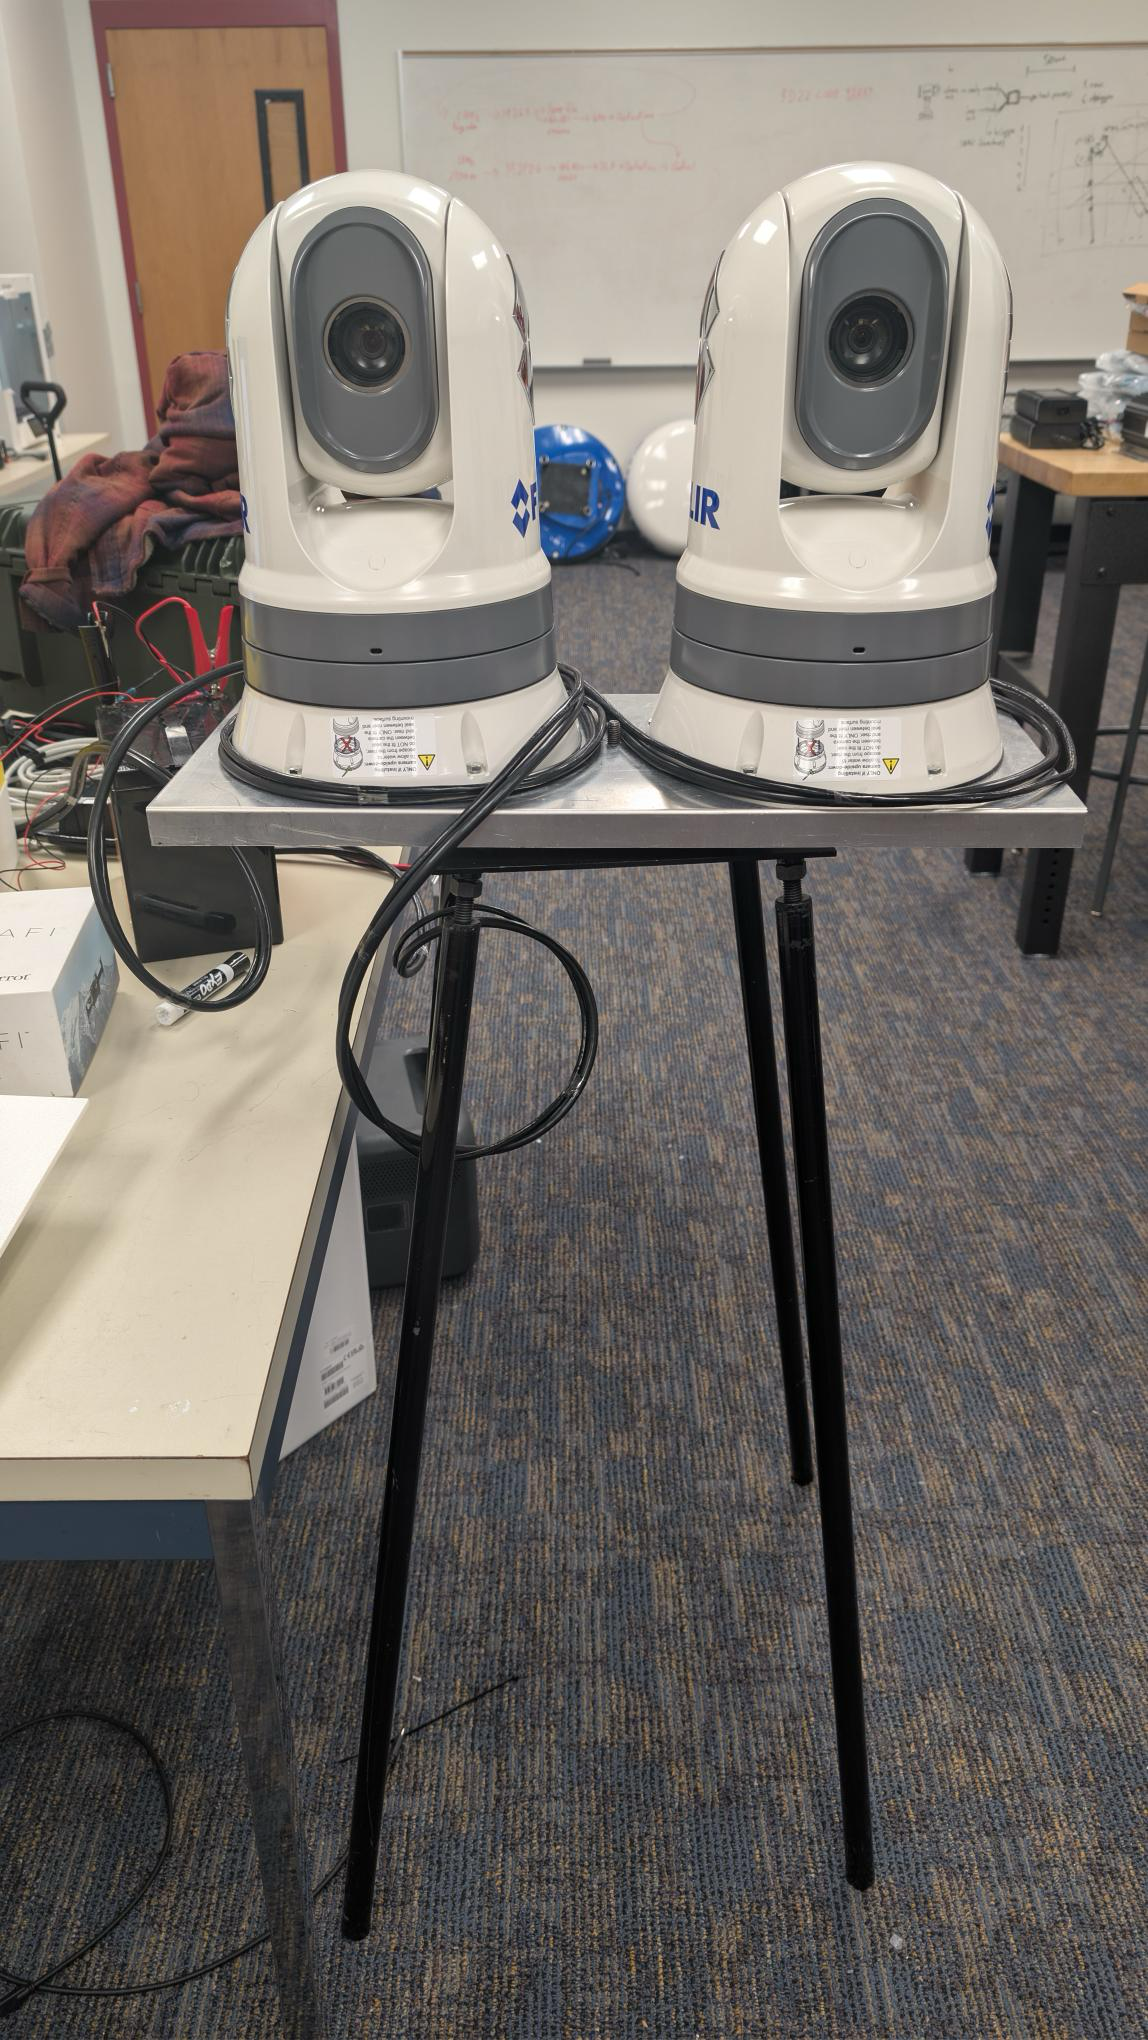
\includegraphics[width=0.95\textwidth]{image_01.png}
\caption*{\scriptsize Two FLIR M300C cameras mounted on 0.9 m stand}
\end{figure}
\end{columns}
\end{frame}

% --- SLIDE 3: SOFTWARE ARCHITECTURE ---
\begin{frame}{Software Architecture: Three-Layer Design}
\begin{center}
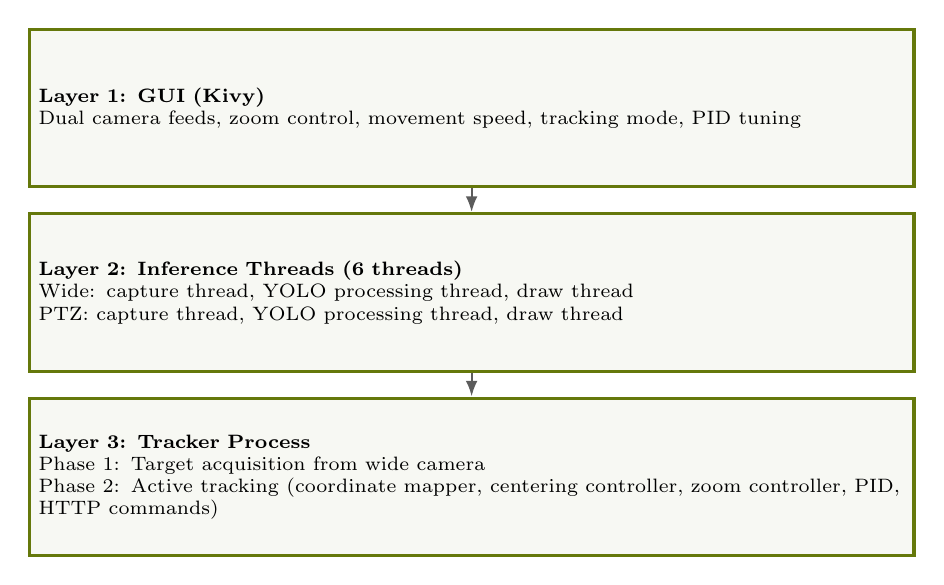
\begin{tikzpicture}[
    every node/.style={font=\scriptsize},
    box/.style={rectangle, draw=Black90, fill=white, text width=2.5cm, minimum height=0.8cm, align=center, line width=0.8pt},
    layer/.style={rectangle, draw=Horseshoe, fill=Horseshoe!5, text width=11cm, minimum height=2.0cm, align=left, line width=1.2pt},
    arrow/.style={->, >={Latex[length=2mm, width=1.5mm]}, draw=Black70, line width=0.8pt}
]

% Layer 1
\node[layer] (L1) at (0,0) {%
\textbf{Layer 1: GUI (Kivy)}\\
Dual camera feeds, zoom control, movement speed, tracking mode, PID tuning
};

% Layer 2
\node[layer, below=0.3cm of L1] (L2) {%
\textbf{Layer 2: Inference Threads (6 threads)}\\
Wide: capture thread, YOLO processing thread, draw thread\\
PTZ: capture thread, YOLO processing thread, draw thread
};

% Layer 3
\node[layer, below=0.3cm of L2] (L3) {%
\textbf{Layer 3: Tracker Process}\\
Phase 1: Target acquisition from wide camera\\
Phase 2: Active tracking (coordinate mapper, centering controller, zoom controller, PID, HTTP commands)
};

\draw[arrow] (L1.south) -- (L2.north);
\draw[arrow] (L2.south) -- (L3.north);

\end{tikzpicture}
\end{center}

\textbf{Key Feature:} Automatic fallback to wide-camera tracking if PTZ loses detection; resumes PTZ control on reacquisition
\end{frame}

% --- SLIDE 4: CALIBRATION AND CROSS-VIEW GEOMETRY ---
\begin{frame}{Calibration and Cross-View Geometry}
\begin{columns}[T]
\column{0.55\textwidth}
\textbf{Bearing Transfer (wide to PTZ):}

\vspace{0.3em}
{\small
Bearing from wide detection $(u,v)$:
\[
\hat{d}_w = \frac{K_w^{-1}\begin{bmatrix}u\\v\\1\end{bmatrix}}{\left\|K_w^{-1}\begin{bmatrix}u\\v\\1\end{bmatrix}\right\|}
\]

Transform to PTZ base frame:
\[
\hat{d}_p = R_{pw}\hat{d}_w
\]

PTZ pan/tilt commands:
\[
\theta = \mathrm{atan2}(\hat{d}_{p,y}, \hat{d}_{p,x})
\]
\[
\phi = \mathrm{atan2}\left(\hat{d}_{p,z}, \sqrt{\hat{d}_{p,x}^2+\hat{d}_{p,y}^2}\right)
\]
}

\column{0.45\textwidth}
\textbf{Zoom Selection by Angular Size:}

\vspace{0.3em}
{\small
Angular height from wide detection:
\[
\alpha \approx \frac{h^w}{f_w}
\]

Desired PTZ pixel height:
\[
h^p_{\mathrm{des}} \approx \frac{h^w}{f_w} f_p(z)
\]

Select zoom $z$ to match $f_p(z)$
}

\vspace{0.5em}
\textbf{Key Property:}
\begin{itemize}
\item Direction-only transfer sufficient for distant targets (no range estimation needed)
\end{itemize}
\end{columns}
\end{frame}

% --- SLIDE 5: SLEW-TO-CLASSIFICATION CONTROL ---
\begin{frame}{Slew-to-Classification Control}
\begin{columns}[T]
\column{0.5\textwidth}
\textbf{Five-State Machine:}
\begin{center}
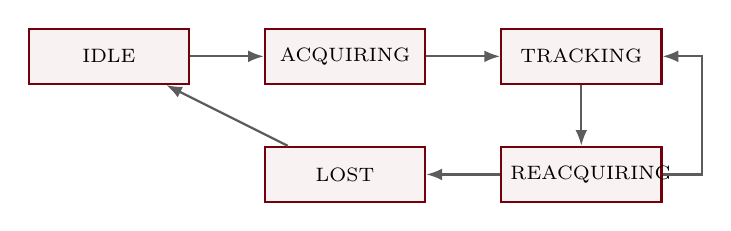
\begin{tikzpicture}[
    state/.style={rectangle, draw=Garnet, fill=Garnet!5, text width=1.8cm, minimum height=0.7cm, align=center, font=\scriptsize, line width=0.8pt},
    arrow/.style={->, >={Latex[length=2mm, width=1.5mm]}, draw=Black70, line width=0.8pt}
]
\node[state] (IDLE) at (0,0) {IDLE};
\node[state] (ACQ) at (3,0) {ACQUIRING};
\node[state] (TRACK) at (6,0) {TRACKING};
\node[state] (REACQ) at (6,-1.5) {REACQUIRING};
\node[state] (LOST) at (3,-1.5) {LOST};

\draw[arrow] (IDLE) -- (ACQ);
\draw[arrow] (ACQ) -- (TRACK);
\draw[arrow] (TRACK) -- (REACQ);
\draw[arrow] (REACQ) -- (LOST);
\draw[arrow] (LOST) -- (IDLE);
\draw[arrow] (REACQ.east) -- ++(0.5,0) |- (TRACK.east);
\end{tikzpicture}
\end{center}

\vspace{0.5em}
\textbf{PID Controller (30 Hz):}
\begin{itemize}
\item $K_p = 1.5$, $K_i = 0.05$, $K_d = 1.0$
\item Inverse-square speed scaling with zoom
\item 2\% centering deadzone
\item Max PTZ speed: 30 deg/s
\end{itemize}

\column{0.5\textwidth}
\textbf{Predictive Bearing Compensation:}

\vspace{0.3em}
{\small
Constant-velocity model with EMA smoothing ($\alpha = 0.3$):
\[
\mathbf{v}_t = \alpha\,\mathbf{v}_{t-1} + (1-\alpha)\,\mathbf{v}_{\mathrm{inst}}
\]

Predicted bearing at command arrival:
\[
\hat{d}_w(t+\Delta) = d_w(t) + \mathbf{v}_t \cdot \Delta
\]
}

\vspace{0.5em}
\textbf{Triggering Policy:}
\begin{itemize}
\item Largest detected target with confidence $> 0.40$
\item Sequential processing (one PTZ resource)
\item 10 s acquisition timeout
\end{itemize}
\end{columns}
\end{frame}

% --- SLIDE 6: AUTOMATED DATASET CONSTRUCTION ---
\begin{frame}{Automated Dataset Construction}
\begin{columns}[T]
\column{0.55\textwidth}
\textbf{Label Transfer Pipeline:}
\begin{enumerate}
\item Wide camera detects ambiguous targets
\item PTZ slews and zooms to verify optically
\item PTZ detector confirms target class ($> 0.35$ confidence)
\item Map PTZ bounding box back to wide view
\end{enumerate}

\vspace{0.5em}
\textbf{Direction-Only Projection:}
{\small
\[
\hat{d}^w_k = R_{wp}\hat{d}^p_k
\]
\[
\begin{bmatrix}u^w_k\\v^w_k\\1\end{bmatrix} \propto K_w \hat{d}^w_k
\]
}

\column{0.45\textwidth}
\textbf{Quality Gates:}
\begin{itemize}
\item PTZ confidence $> 0.35$ (track threshold)
\item Class agreement (wide vs PTZ)
\item Motion blur check (Laplacian variance)
\item Exposure saturation check
\item Frame-boundary rejection
\end{itemize}

\vspace{0.5em}
\textbf{Dataset Schema:}
\begin{itemize}
\item Wide frame or short clip
\item Transferred bounding box
\item PTZ telemetry ($\theta, \phi, z$)
\item Detector scores (wide + PTZ)
\item Quality metrics
\end{itemize}
\end{columns}
\end{frame}

% --- SLIDE 7: RESULTS - THROUGHPUT ---
\begin{frame}{Results: Detector Throughput}
\begin{columns}[T]
\column{0.5\textwidth}
\textbf{Parallel GPU/DLA Inference:}

\vspace{0.3em}
\begin{table}[h]
\centering
\scriptsize
\begin{tabular}{@{}lcc@{}}
\toprule
\textbf{Camera} & \textbf{Wide (GPU)} & \textbf{PTZ (DLA)} \\
\midrule
Model & YOLOv11s & YOLOv11n \\
Resolution & 1024$\times$1024 & 640$\times$640 \\
Inference (ms) & 27.9 & 46.5 \\
Throughput (FPS) & \textcolor{Atlantic}{\textbf{35.9}} & \textcolor{Atlantic}{\textbf{21.5}} \\
Detection rate & 100\% & 99\% \\
Avg confidence & 0.553 & 0.529 \\
\bottomrule
\end{tabular}
\end{table}

\vspace{0.5em}
\textbf{Aggregate throughput:} \textcolor{Rose}{\textbf{57.4 FPS}}

\vspace{0.3em}
True parallel execution (no GPU time-slicing)

\column{0.5\textwidth}
\textbf{Codec Impact on Latency:}

\vspace{0.3em}
\begin{itemize}
\item \alert{H.264:} 2--4 frames decode buffering\\(66--133 ms latency)
\item \alert{MJPEG:} Independent frame encoding\\(<5 ms decode latency)
\item \textbf{Savings:} 60--130 ms reduction
\end{itemize}

\vspace{0.5em}
\textbf{Key Insight:}
\begin{itemize}
\item GPU 2.2--2.8$\times$ faster than DLA per model
\item DLA eliminates CUDA context switch overhead
\item Enables true concurrent inference
\end{itemize}
\end{columns}
\end{frame}

% --- SLIDE 8: RESULTS - DRONE TRACKING DEMO ---
\begin{frame}{Results: Drone Tracking Demonstration}
\begin{columns}[T]
\column{0.6\textwidth}
\begin{figure}
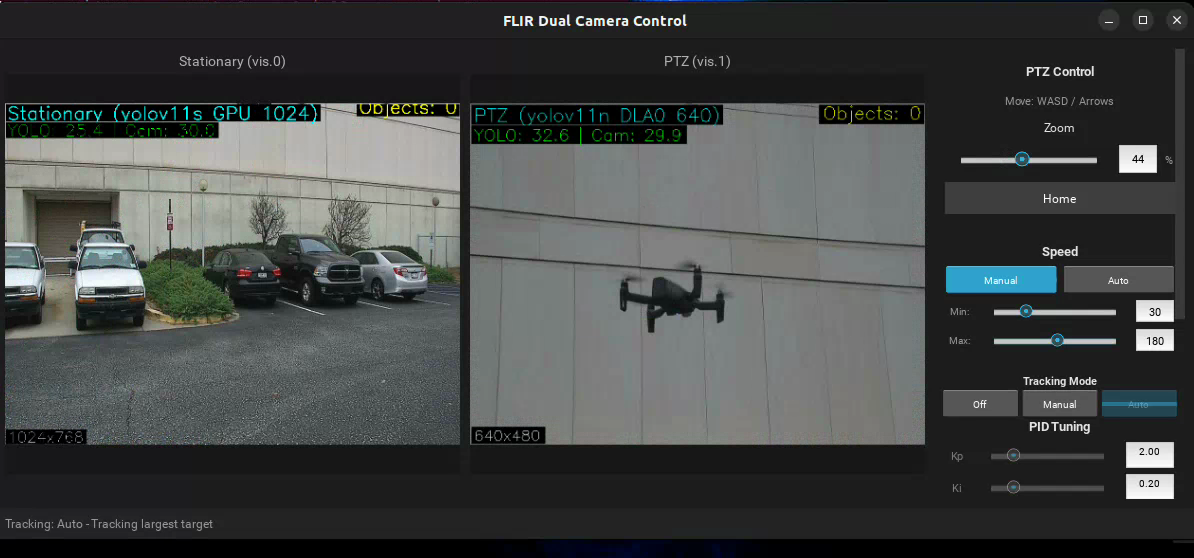
\includegraphics[width=\textwidth]{fig_gui_dual_feed.png}
\caption*{\scriptsize Live GUI during 42-second drone tracking test}
\end{figure}

\column{0.4\textwidth}
\textbf{Test Parameters:}
\begin{itemize}
\item Duration: 42 seconds
\item Total frames: \textasciitilde{}42,000 (both cameras)
\item Target: Small commercial drone
\item \alert{Zero reacquisitions} (continuous lock)
\end{itemize}

\vspace{0.5em}
\textbf{Performance:}
\begin{itemize}
\item Wide detection: 100\% rate
\item PTZ detection: 99\% rate
\item Smooth state transitions:\\IDLE $\to$ ACQUIRING $\to$ TRACKING
\item PID maintained stable centering throughout
\end{itemize}
\end{columns}
\end{frame}

% --- SLIDE 9: RESULTS - RESOLUTION COMPARISON ---
\begin{frame}{Results: Resolution Comparison}
\begin{columns}[T]
\column{0.5\textwidth}
\begin{figure}
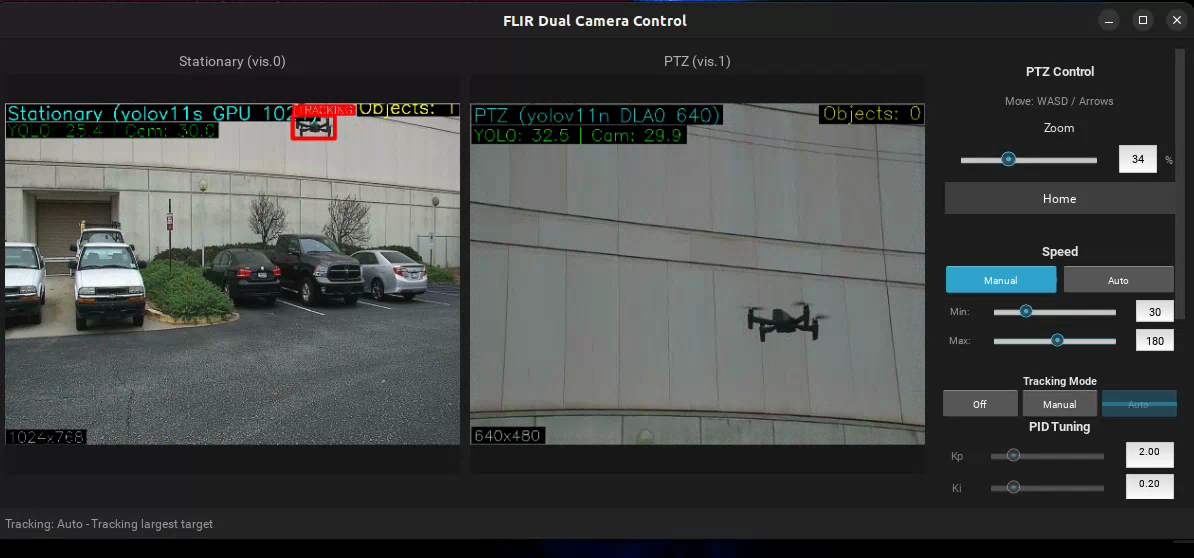
\includegraphics[width=0.9\textwidth]{fig_drone_tracking.png}
\caption*{\scriptsize PTZ zoomed view: \textasciitilde{}120$\times$90 px}
\end{figure}

\textbf{PTZ View Benefits:}
\begin{itemize}
\item 6$\times$ linear resolution gain
\item Moves target into high-accuracy regime (99.1\% mAP50)
\item Optical ground truth (no hallucination)
\end{itemize}

\column{0.5\textwidth}
\textbf{Resolution Analysis:}

\vspace{0.3em}
\begin{block}{Wide-Angle View}
\begin{itemize}
\item Target size: \textasciitilde{}20$\times$15 px
\item Insufficient for classification
\item Distractors indistinguishable
\end{itemize}
\end{block}

\vspace{0.3em}
\begin{block}{PTZ Zoom View (35--45\%)}
\begin{itemize}
\item Target size: \textasciitilde{}120$\times$90 px
\item 6$\times$ linear increase
\item Clear structural detail
\end{itemize}
\end{block}

\vspace{0.5em}
\textbf{Key Advantage:} Optical zoom provides \emph{true} high-resolution data, not generative reconstruction
\end{columns}
\end{frame}

% --- SLIDE 10: SYSTEM INTEGRATION ---
\begin{frame}{System Integration: Dual-Instance Pipeline}
\begin{figure}
\centering
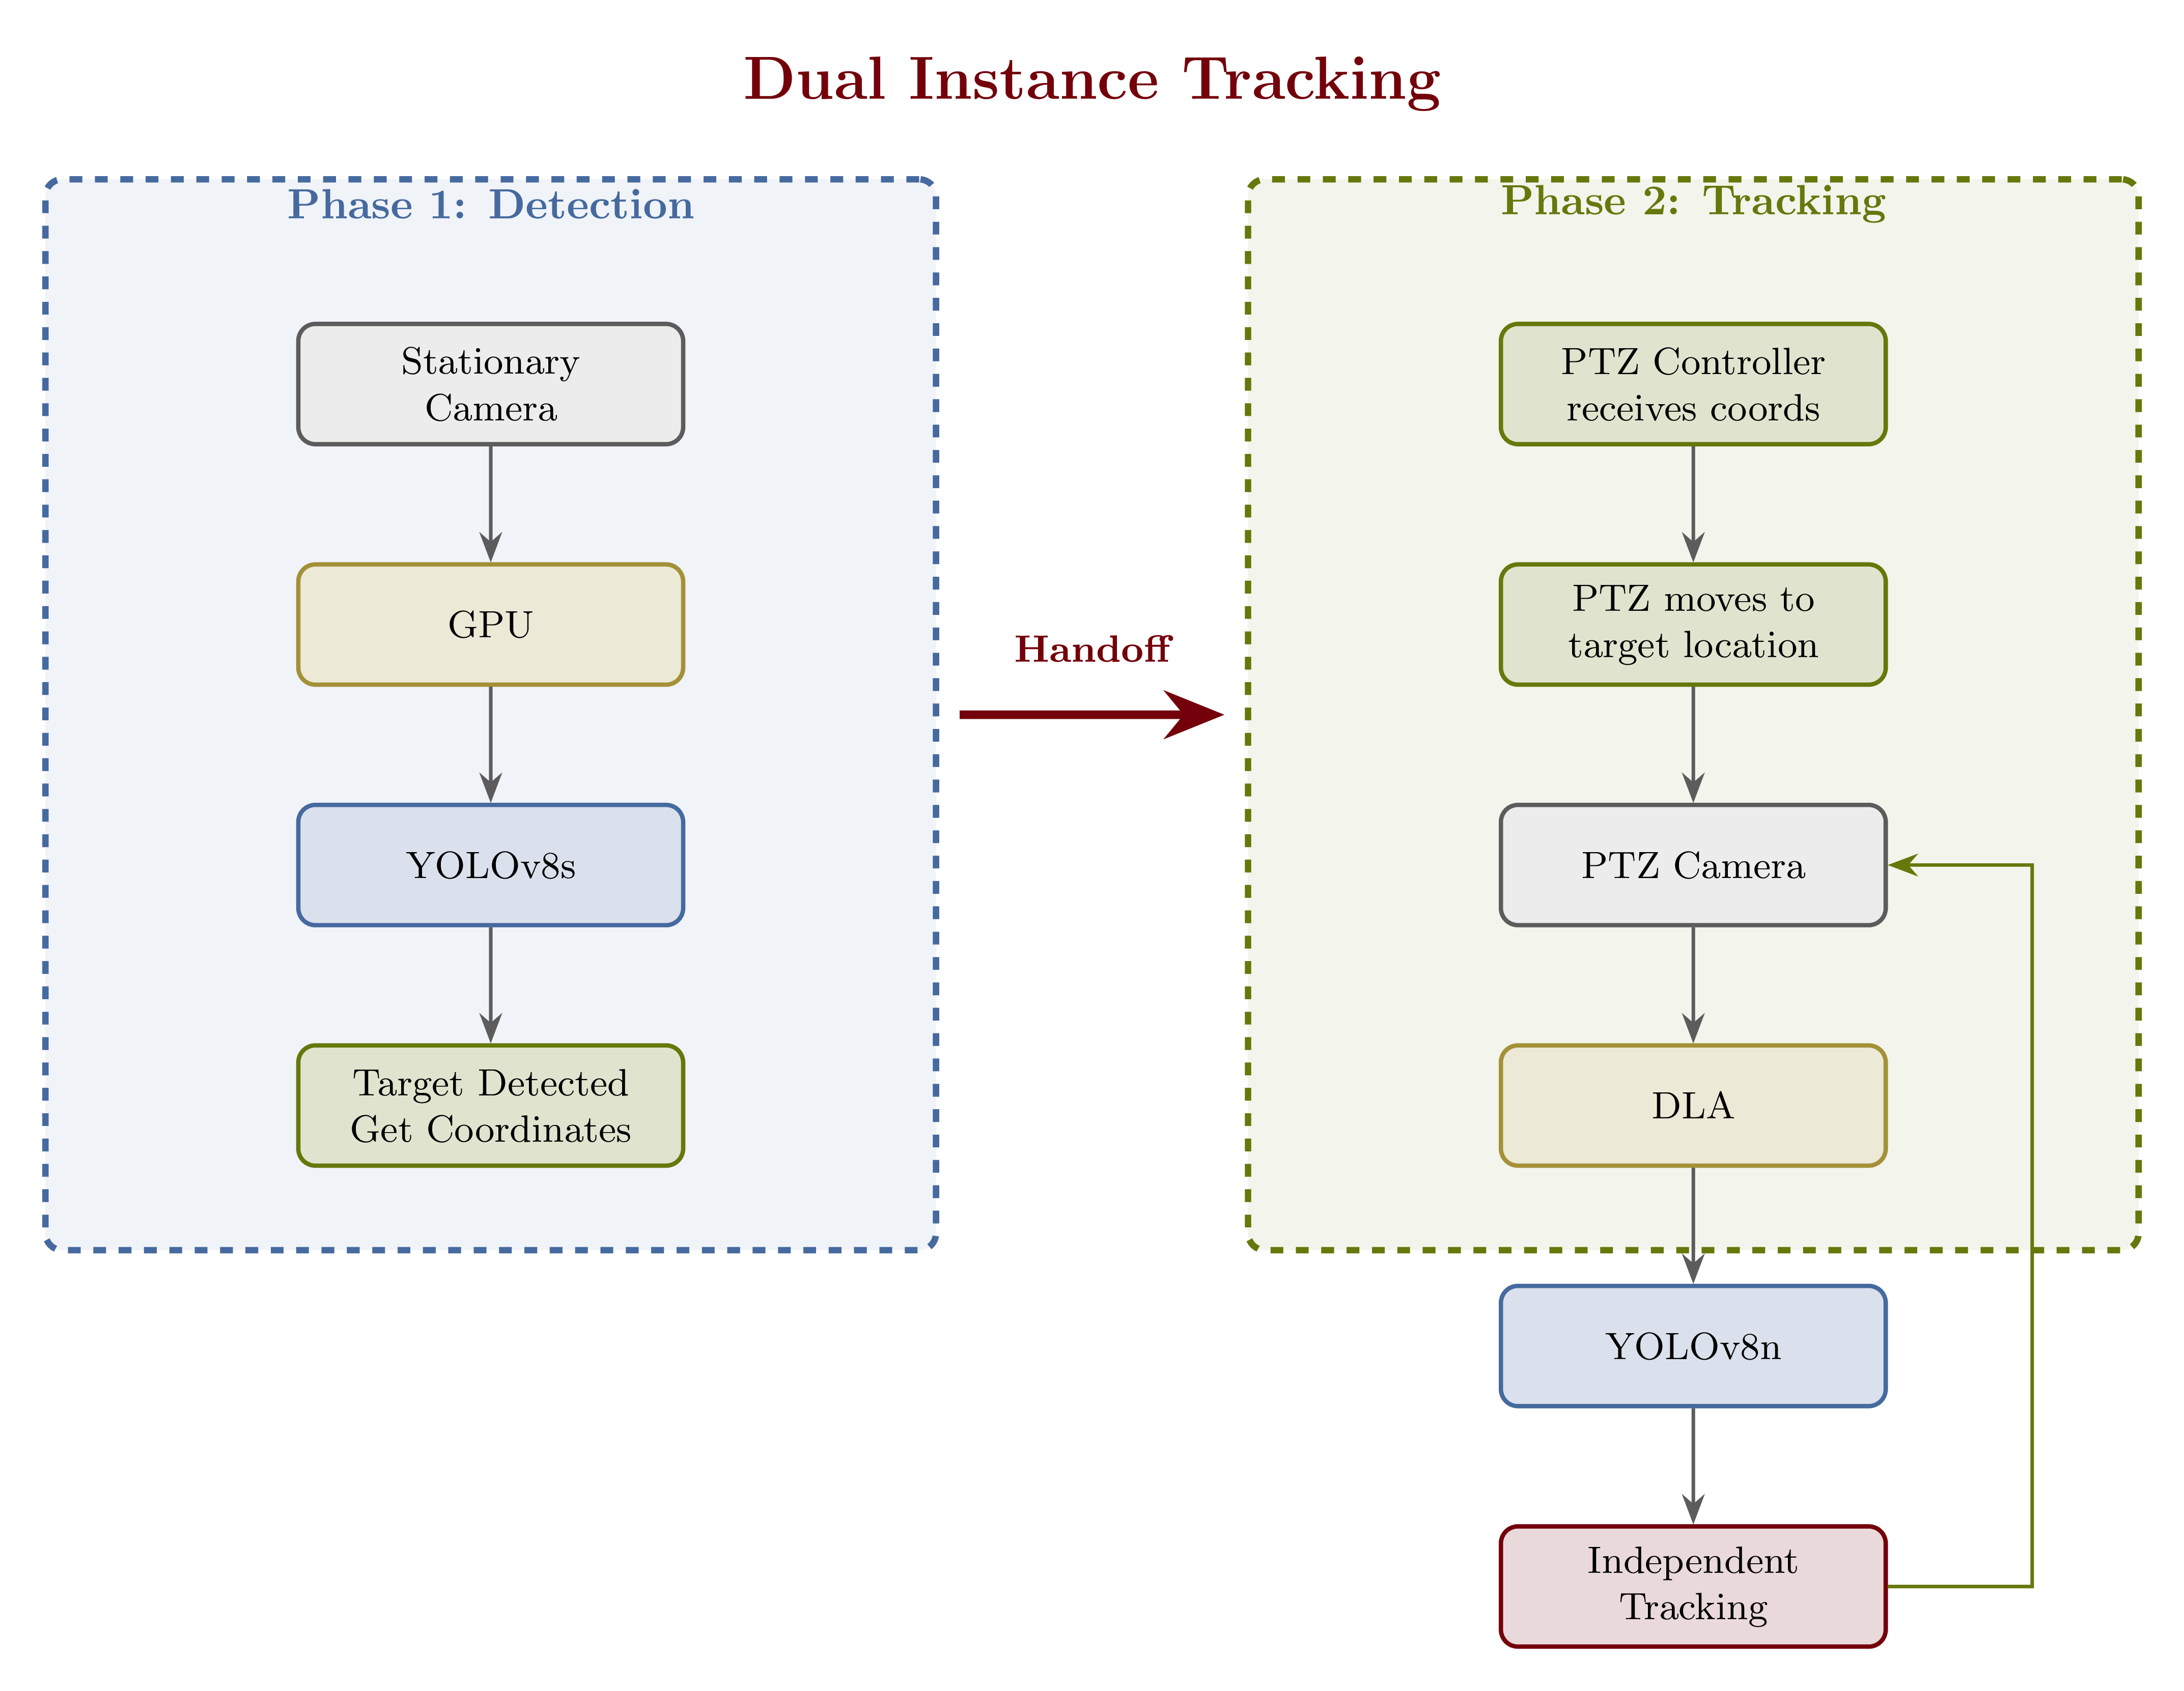
\includegraphics[width=0.85\textwidth]{image_02.png}
\caption*{\scriptsize Dual-instance tracking pipeline: Wide detector on GPU, PTZ detector on DLA}
\end{figure}

\textbf{Pipeline Features:}
\begin{itemize}
\item Concurrent detection streams (no resource contention)
\item Automatic state machine management (5 states)
\item Real-time label transfer with quality gates
\item Battery-powered for field deployment
\end{itemize}
\end{frame}

% --- SLIDE 11: CONCLUSIONS AND FUTURE WORK ---
\begin{frame}{Conclusions and Future Work}
\begin{columns}[T]
\column{0.5\textwidth}
\textbf{Contributions:}
\begin{itemize}
\item Dual-camera system for automated small-object dataset construction
\item Predictive slew-to-classification control framework
\item Parallel GPU/DLA inference (57.4 FPS aggregate)
\item Validated on 42-second drone tracking demonstration
\end{itemize}

\vspace{0.5em}
\textbf{Key Results:}
\begin{itemize}
\item 6$\times$ resolution gain via optical zoom
\item 100\% wide detection rate, 99\% PTZ detection rate
\item MJPEG codec reduces latency by 60--130 ms
\item Zero reacquisitions during continuous tracking
\end{itemize}

\column{0.5\textwidth}
\textbf{Current Limitations:}
\begin{itemize}
\item Single PTZ (no multi-target zoom)
\item Potential loss during slew for fast targets
\item Small-parallax assumption for label transfer
\end{itemize}

\vspace{0.5em}
\textbf{Future Work:}
\begin{itemize}
\item Label quality evaluation vs manual annotation
\item Custom YOLO models trained on FGVC aircraft data
\item Benchmark COCO vs domain-specific weights
\item Multi-PTZ scheduling for higher throughput
\item Field deployment with extended battery testing
\end{itemize}
\end{columns}
\end{frame}

% --- QUESTIONS SLIDE ---
{
\setbeamercolor{background canvas}{bg=Garnet}
\setbeamercolor{normal text}{fg=white}
\usebeamercolor[fg]{normal text}
\begin{frame}[plain]
\vfill
\begin{center}
{\Huge\textbf{Questions?}}\\[2em]
{\Large J. Wang, J.C. Vaught, D. Cahl, Y. Wang}\\[0.5em]
{\normalsize Department of Mechanical Engineering\\University of South Carolina}\\[1.5em]
{\normalsize\texttt{jvaught@sc.edu}}
\end{center}
\vfill
\end{frame}
}

\end{document}
